\chapter{Methodology}
\label{chap:methods}

With this thesis, we aim to measure and compare the LLM inference performance and energy efficiency of a diverse set of accelerated servers across multiple deployment scenarios. However, the heterogeneity of models, hardware, and software stacks, as well as the numerous interacting factors that influence performance, makes this task non-trivial. To structure our analysis, we begin by identifying the principal factors that impact LLM inference performance, focusing on four key elements:

\begin{itemize}
\item \textbf{Sequence length}: the number of input and output tokens generated. We ensure consistency by using the same inference dataset (Section \ref{chap:methods:sec:dataset}) for all experiments.
\item \textbf{Model architecture}: the characteristics of the LLM being served. We address the heterogeneity of LLM models by evaluating a diverse set of popular open-source models and examining their characteristics in relation to performance. In particular, we analyze:
\begin{itemize}
\item \textbf{Model Size}: the total number of model parameters;
\item \textbf{Sparsity}: the proportion of parameters that are sparsely activated, in the case of Mixture-of-Experts (MoE) models.
\item \textbf{Quantization}: the numerical format used for model weights and activations. Wherever supported, we compare 16-bit precision with 8-bit precision.
\end{itemize}
\item \textbf{Parallelism}: The number of sequences processed in parallel (\textbf{batch size}) and the number of devices used for inference greatly impact performance, depending on the parallel serving strategy chosen (\textbf{Data, Pipeline, Tensor or Expert Parallelism}).
\item \textbf{Inference Engine}: the software stack influences performance. We maintain consistency by using the same inference engine (vLLM \cite{kwon2023efficient}) across all the GPU servers. Dataflow accelerators, on the other hand, require an architecture-specific engine.
\end{itemize}

\section{LLM Inference Performance}
\label{chap:methods:sec:model}

In Section \ref{chap:background:sec:llms}, we introduced the typical decoder-only transformer architecture, which consists of a stack of layers that includes a self-attention block and a feed-forward network. While Section \ref{chap:background:sec:serving} discusses how these models are used for generating text outputs. In this section, we provide a detailed description of LLM inference, discussing how the four factors identified earlier affect the computational and memory workload.
This analysis enables us to critically analyze the results presented in Chapter \ref{chap:results}, understanding the distance between ideal and practical performance trends.

As discussed in Section \ref{chap:background:sec:serving}, an inference task requires processing the entire prompt during the prefill phase. Then, in the decode phase, a new token is generated per forward pass.
This meas that the total latency of the inference job can be identified as $\Delta t = \Delta t_{FP} \times(FP_{IN} + FP_{OUT})$, where $\Delta t_{FP}$ is the latency of the forward pass, $FP_{IN}$ is the number of forward passes needed for the prefill phase (typically 1), and $FP_{OUT}$ corresponds to the number of output tokens.

$\Delta t_{FP}$ depends on the specific software implementation and hardware accelerator that are being employed. But, in general, we can decompose it in two parts: $\Delta t_{FP} = \Delta t_{C} + \Delta t_{mem}$, where $\Delta t_{C}$ is related to the computation, and $\Delta t_{mem}$ is related to memory accesses.
With an accelerator with a throughput of $TP\  \text{OPs}/s$ and has a memory bandwidth of $BW\ \text{bytes}/s$, $\Delta t_{C} = C_{\text{forward}}/TP$ and $\Delta t_{C} = Mem/BW$, where $C_{\text{forward}}$ and $Mem$ are the number of operations and the amount of memory to access at each forward pass. 

By applying the formula proposed by Kaplan et al.~\cite{kaplan2020scaling}, we can estimate the forward-pass computational cost \( C_{\text{forward}} \) in terms of the language model architecture and the context length. Specifically, we characterize a model by its total parameter count \( N \), the number of layers \( n_\text{layer} \), the dimensionality of the attention layer output \( n_\text{model} \), and the number of attention head groups $ n_\text{groups}$.

For a model with size \( N \), the computational cost per forward pass can be approximated as
\[
C_{\text{forward}} \approx 2N + 2n_\text{layer} n_{\text{ctx}} d_{\text{attn}}.
\]

The first term refers to the context-independent FLOPs, which are related to the matrix-matrix multiplications associated with the $W^Q$, $W^K$, and $W^V$ projection matrices, as well as the feed-forward block. The second term, however, is context-dependent, as it scales linearly with the context length.
Kaplan et al.~\cite{kaplan2020scaling} argue that the context-independent component of the computation dominates the overall cost, enabling a simplification of the forward-pass complexity to $C_{\text{forward}} \approx 2N$, where the number of FLOPs scales linearly with the model size $N$.

To evaluate the validity of this hypothesis, we explicitly compute the FLOPs associated with both the context-dependent and context-independent components across five open-source models of varying sizes, selected from those used in our experimental evaluation. Table~\ref{tab:context_architecture} illustrates the relative contribution of these two components for different context lengths and increasing model scales. We observe that smaller models exhibit a larger relative impact from context-dependent operations. Nevertheless, for moderate context lengths (fewer than $10{,}000$ tokens), more than $85\%$ of the total computational cost consistently arises from the context-independent component across all models. This empirical evidence supports the robustness of the linear scaling trend for inputs of this size.

\begin{table}[h]
\centering
\caption{Percentage of context-independent FLOPs over total for different context lengths.}
\label{tab:context_architecture}
\begin{tabular}{lccccccc}
\toprule
\textbf{Model} & \textbf{Params} & \textbf{Layers} & \textbf{Hidden} &
\textbf{100} & \textbf{1,000} & \textbf{10,000} & \textbf{100,000} \\
\midrule
\textbf{Llama 3.1 8B}  & 8B      & 32 & 4096 & 99.8\% & 98.4\% & 85.9\% & 37.9\% \\
\textbf{Qwen3 14B}     & 14.8B   & 40 & 6144 & 99.9\% & 98.8\% & 89.5\% & 46.1\% \\
\textbf{Qwen3 32B}     & 32B     & 64 & 8192 & 99.9\% & 99.2\% & 92.4\% & 55.0\% \\
\textbf{Nemotron 49B}  & 49B     & 80 & 8192 & 99.9\% & 99.3\% & 93.7\% & 59.9\% \\
\textbf{Llama 3.3 70B} & 70B     & 80 & 8192 &100.0\% & 99.5\% & 95.5\% & 68.1\% \\
\bottomrule
\end{tabular}
\end{table}

Introducing parallelism across multiple sequences complicates the analysis: with a batch size $b$, each sequence requires $C_{\text{forward}}$ operations. If we neglect the context-dependent portion of the computation that differs across sequences, the total compute latency scales linearly with batch size,
\[
\Delta t_{C}(b) = b \times \Delta t_{C}(1),
\]
implying that the number of FLOPs per token remains constant for different values of $b$.
Memory accesses, instead, display a different behavior. The amount of memory (\( \text{Mem} \)) that is read at each forward pass consists of two parts: a context-independent component (the model’s weights) and a context-dependent component (the KV cache).  
For a sequence of length $n_{\text{ctx}}$ and a batch size $b$ the total amount of memory to read is
\[
Mem = NP_W + 2bn_\text{layer} n_{\text{ctx}} \frac{ d_{\text{model}} }{n_{\text{groups}}} P_A
\]
where $P_W$ is the number of bytes per weight, and $P_A$ is the number of bytes per value in the KV cache.
It is essential to note that, unlike computation, the amount of memory allocated per token is not constant with respect to the batch size, as access to the model weights is shared among all the sequences in the batch.

Using 1024 tokens as an example, we observe that for small batch sizes the contribution of the KV cache to the total memory footprint is negligible ($0.1\%$–$0.2\%$ across model sizes for $b=1$). However, as the batch size increases, the KV cache occupies a growing fraction of memory, particularly for smaller models, reaching $7.1\%$–$21.2\%$ at a batch size of $128$.

Once the number of operations and the memory footprint are identified, we have all the elements to compute the latency $\Delta t_{FP}$ under an idealized model:
\[
\Delta t_{FP} = \Delta t_{C} + \Delta t_{mem} = \frac{(2N + 2n_\text{layer} n_{\text{ctx}} d_{\text{attn}})b}{TP} + \frac{NP_W + 2bn_\text{layer} n_{\text{ctx}} \frac{ d_{\text{model}}}{n_{\text{groups}}} P_A}{BW} \approx \frac{2N}{TP} + \frac{NP_W}{BW}
\]
Where the approximation holds for $N >> b n_{\text{ctx}} d_{\text{model}}n_\text{layer}$.

This simplified model allows us to highlight some trends in the theoretical performance of LLM inference.

First of all, we can relate the latency to the size of the model. We can expect \textbf{latency to scale linearly with the model size $N$}, as both computation and memory access-related latencies are dominated by that factor.

Second, we can predict the \textbf{impact of quantization} on performance. In fact, weight quantization affects $P_W$, reducing $\Delta t_{Mem}$, while activation quantization affects both $P_A$ and $TP$, reducing both $\Delta t_{Mem}$ and $\Delta t_{C}$.

Third, we can study the \textbf{impact of batch size on operational intensity $OI$}. Expressed in FLOPs/byte, it measures the ratio between operations and memory accesses. Using our model, it can be defined as:
\[
OI=\frac{(2N + 2n_\text{layer} n_{\text{ctx}} d_{\text{attn}})b}{NP_W + 2bn_\text{layer} n_{\text{ctx}} \frac{ d_{\text{model}}}{n_{\text{groups}}} P_A} \approx \frac{2N}{NP_W}b = \frac{2}{P_W}b
\]
We notice that, in the approximated performance model, \textbf{operational intensity scales linearly with batch size}, and it is independent of model size.
\begin{comment}
\ref{fig:roofline} shows how our experimental data on Llama 3.1 8B compares with two different versions of the performance model. In orange, we have the ideal performance model, which uses the theoretical peak $TP$ and $BW$, as provided by the vendor. The scaled model (in blue) estimates the actual $BW$ and $TP$ by choosing the values that best approximate the experimental data points.

\begin{figure}[H]
    \centering
    \includegraphics[width=\textwidth]{figs/roofline.pdf}
        \caption{Roofline model of Llama 3.1 8B on NVIDIA GPUs.}
    \label{fig:roofline}
\end{figure}

We notice that, for small ($\le16$) batch sizes, the scaled performance model accurately predicts performance, while it overestimates performance for large batch sizes. This is due to the dynamicity of vLLM batch size, which is downscaled automatically to prevent out-of-memory errors when batching long sequences.
\end{comment}

Finally, we can use this model to understand a well-known \textbf{limitation of LLM inference: its memory-bound nature}. In fact, especially for small batch sizes (low $OI$), the impact of throughput on performance is negligible compared to that of memory bandwidth. As discussed in Chapter \ref{chap:hardware}, the throughput of modern GPUs is in the hundreds or thousands of TFLOPs ($10^{14}-10^{15}$ FLOPs), while memory bandwidth is in the TBytes/s ($10^{12}$).
This means that the operational intensity necessary to achieve peak performance is between $ 10^2$ and $10^3$ FLOPS/byte, highly favoring large batch sizes.

\subsection{Mixture of Experts}
\label{chap:model:sec:moe}

In the previous section, we analyzed the performance of dense decoder-only LLMs. To model the performance of Mixture-of-Experts (MoE) models, we have to consider their sparsity.
We indicate the number of active parameters of Mixture of Experts Models with $A$, and we define sparsity as $S=A/N$.

A batch size of one indicates the trivial case. We can simply substitute $N$ for $A$, obtaining a theoretical performance improvement of $Speedup_1 = 1/S$.

\[
\Delta t_{FP} = \Delta t_{C} + \Delta t_{mem} = \frac{(2A + 2n_\text{layer} n_{\text{ctx}} d_{\text{attn}})b}{TP} + \frac{AP_W + 2bn_\text{layer} n_{\text{ctx}} \frac{ d_{\text{model}}}{n_{\text{groups}}} P_A}{BW} \approx \frac{2A}{TP} + \frac{AP_W}{BW}
\]

Increasing batch size complicates the problem, as each sequence uses a different set of experts.
A model with $E_{tot}$ experts, of which $E_{act}$ are active, $b$ will activate $E_{act}$ experts for each sequence in the batch. Notably, the sets of active experts overlap, so the experts that are active across the batch are between $E_{act}$ and $\min(bE_{act},E_{tot})$.
In this case, each sequence requires approximately $2A$ FLOPS/token ($1/S \times$ speedup), while the amount of memory ($\text{Mem}$) read at each forward pass depends on the total number of active experts. 

\subsection{Multi-Device}
\label{chap:model:sec:multi}

In Section \ref{chap:background:sec:serving}, we introduced four techniques to parallelize multi-GPU inference: Pipeline Parallelism (PP), Tensor Parallelism (TP), Expert Parallelism (EP), and Data Parallelism (DP).
In this section, we describe how our performance model can be adapted for multi-device inference. To do so, we build on the contribution of Subramanian et al. \cite{subramanian2024comprehensive}.

To compute the speedup that is possible to achieve with parallelization, we use the formula:

\[
 S = \frac{ITL \cdot S^* +OH}{ITL}
\]

Where $OH$ is the overhead caused by GPU-to-GPU communication. The lower bound of the overhead is constituted by the amount of memory that needs to be moved $Vol$ divided by the bandwidth of the GPU-to-GPU network $BW_{Net}$:  $OH = Vol/BW_{Net}$. 

Each parallelization technique leads to different values of $TP$, $BW$, $Vol$, and contributes to increasing memory capacity in a different way.

\begin{comment}
    \ref{tab:parall} summarizes those contributions.

\begin{table}[H]
\centering
\footnotesize
\caption{Speedup across parallelization techniques.}
\begin{tabularx}{\textwidth}{@{}c c c c c@{}}
\toprule
\textbf{Technique} & \textbf{Throughput ($TP$)} & \textbf{Bandwidth ($BW$)} &
\textbf{Volume ($Vol$)} & \textbf{Mem. Size} \\
\midrule
\textbf{Data Parallel}     & $\times D$                             & $\times D$                           & $0$                                         & $\times 1$ \\
\textbf{Pipeline Parallel} & $\times 1$                             & $\times 1$                           & $b\, d_{\text{model}} D$                      & $\times D$ \\
\textbf{Tensor Parallel}  & $\times D$                             & $\times D$                           & $4b\, n_{\text{layers}}\,d_{\text{model}}\,P_A\,D$ & $\times D$ \\
\bottomrule
\end{tabularx}
\label{tab:parall}
\end{table}
\end{comment}

\begin{itemize}
    \item \textbf{Data Parallelism}: Data Parallelism simply replicates the single-device setting $D$ times, increasing throughput and memory bandwidth linearly ($TP_D=D\cdot TP, BW_D=D\cdot BW$). There is no GPU-to-GPU communication, so $OH=0$ and the expected speedup is linear $S_D = D$. The only limitations of this technique are that it does not increase the overall memory size available for the weights, and it offers limited speedup when $b < D$, as some devices remain inactive.

    \item \textbf{Tensor parallelism (TP)}: This technique shards the model's weights across devices layer by layer, increasing the memory size by a factor of $D$. As all devices work in parallel, we can also assume that $TP$ and $BW$ increase by a factor of $D$. The volume of data to be moved at every forward pass is $4b n_{\text{layers}}d_{\text{model}} P_A$  \cite{subramanian2024comprehensive}, introducing an overhead $OH$ that depends on the GPU-to-GPU bandwidth $BW_{C2C}$.

    \item \textbf{Expert Parallelism (EP)}: Expert Parallelism works similarly to Tensor Parallelism and thus results in a similar behavior. The key differences are that attention layers are not replicated, and thus the memory scaling is less than $D$, and the load imbalance that is caused by the unpredictable nature of expert activations.

    \item \textbf{Pipeline parallelism} is often used to host large models over multiple nodes. It does not increase compute nor bandwidth, but it requires moving substantially less memory than Tensor Parallelism ($b d_{\text{model}}D << 4b n_{\text{layers}}d_{\text{model}} P_A$).
\end{itemize}

In conclusion, we can expect Data Parallelism to perform best, as it has null overhead. However, when memory size becomes a limiting factor, Pipeline, Tensor, and Expert Parallelism become the preferred solutions.
\section{Experimental Setup}
\label{chap:exp}

In this Section, we describe in detail the experimental setup we used to evaluate LLM inference.
The subsections are organized as follows: 
\ref{chap:methods:sec:metrics} discusses the performance metrics used to compare the different accelerators, 
\ref{chap:methods:sec:dataset} describes the inferense dataset used,
\ref{chap:methods:sec:dataset} describes the inference dataset, and finally \ref{chap:methods:sec:single}, \ref{chap:methods:sec:multi}, and   \ref{chap:methods:sec:dsa} present the methodology of the single-GPU, multi-GPU and dataflow accelerators experiments.
\subsection{Inference Dataset}
\label{chap:methods:sec:dataset}

In the Section \ref{chap:methods:sec:model}, we discussed that the number of input and output tokens directly influences the performance of LLM inference, as it linearly relates to the number of forward passes to be performed, and it influences the context-dependent part of the computation and the size of the KV cache.

To replicate a realistic chatbot scenario in terms of input and output lengths, we use the MLSysChat1M dataset \cite{zheng2023lmsys}, a collection of 1 million real-world, multi-turn conversations with chatbots.
MLSysChat1M uses the OpenAI chat schema, a standard format for API-based inference. Each conversation is represented as a sequence of turns assigned to “user,” “system,” or “assistant” roles.

During preprocessing for our benchmark, we transform chat logs into inference requests by removing the final assistant response from each conversation and setting the output length to match the original response's length. To achieve this, we tokenize the ground-truth response to obtain its exact token count, then constrain generation by setting both the minimum and maximum token limits to this value, ensuring the model produces a reply of identical length.

From the MLSysChat1M dataset, we select the first 1,000 conversations for our analysis, filtering to include only those with a total character count between 64 and 20,000. This range excludes trivial or empty samples while staying within the models’ maximum context length, ensuring that the resulting distribution of prompt and answer lengths remains plausible for evaluating performance and energy efficiency.

\subsection{Performance Metrics}
\label{chap:methods:sec:metrics}
To provide a comprehensive evaluation of LLM inference, we consider both performance and energy efficiency using well-established metrics:
\begin{itemize}
    \item \textbf{End-to-End (E2E) Latency}: The total time required to generate an output sequence. Latency is a primary quality-of-service (QoS) metric, as it reflects the waiting time experienced by end users. Using our performance model, it represents the sum of all the latencies of the forward passes necessary to generate a sequence ($\sum_{i=0}^{T+1} \Delta t_{FP}(i)$).
    \item \textbf{Time To First Token (TTFT)}: The time  taken to produce the first output token. It a the latency of a forward pass which involves a prefill task.
    \item \textbf{Inter Token Latency (ITL)}: Average interval between the generation of two consecutive tokens. It is obtained as $(\text{E2E}-\text{TTFT})/\text{Tokens}_{out}$. It represents the average latency of a forward pass.
    \item \textbf{Throughput}: The number of tokens processed per second. It is obtained as $\text{Tokens}/\text{E2E}$. This is a key metric in a batch-inference scenario, where the goal is to process multiple requests as quickly as possible.
    Considering only output tokens, it can be expressed as $b/\Delta t_{FP}$, assuming a constant batch size $b$. Following prior work \cite{LLMInfbench}, in the experimental evaluation, we consider both input and output tokens.
    \item \textbf{Energy Efficiency}: The number of tokens generated per joule of energy consumed $\text{Tokens}/\text{Energy}$. Energy consumption is measured as the integral of power over time, so it can be reduced by either lowering power consumption or reducing latency. Consistent with throughput, we include both input and output tokens in this metric.
\end{itemize}
\subsection{LLM Models}
\label{chap:methods:sec:models}

In our performance and energy efficiency evaluation, we employ fourteen open-source large language models from the Llama\cite{grattafiori2024llama,meta2025llama4}, Qwen\cite{yang2024qwen2,yang2025qwen3}, Mistral\cite{jiang2024mistral}, and DeepSeek R1\cite{guo2025deepseek} families.
The architectural features of those models are summarized in \ref{tab:models}.
\begin{comment}
\begin{table}[h!]
\centering
\small
\caption{LLMs used in this study: fourteen models and their features.}
\label{tab:models}
\begin{tabular}{|l|cc|cclc|}
\hline
\textbf{Model Name} & \multicolumn{2}{c|}{\textbf{Parameters}} & \textbf{Layers} & \textbf{Attention} & \textbf{FFN Type} & \textbf{Context} \\
 & \textbf{Total} & \textbf{Active} & & & & \\
\hline
\textbf{Llama 3.1 8B} & 8B & = & 32 & GQA (32/8) & Dense & 128K \\
\textbf{Llama 3.3 70B} & 70B & = & 80 & GQA (64/8) & Dense & 128K \\
\textbf{Nemotron Super 49B} & 49B & = & 80 & GQA (64/8) & Dense & 128K \\
\textbf{Llama 4 Scout 17B 16E} & 109B & 17B & 48 & GQA (40/8) & MoE (16E) & 10M \\
\hline
\textbf{Qwen3 8B} & 8.2B & = & 36 & GQA (32/8) & Dense & 128K \\
\textbf{Qwen3 14B } & 14.8B & = & 40 & GQA (40/8) & Dense & 128K \\
\textbf{Qwen3 32B } & 32.8B & = & 64 & GQA (64/8) & Dense & 128K \\
\textbf{Qwen2.5 72B } & 72B & = & 80 & GQA (64/8) & Dense & 128K \\
\textbf{Qwen3 235B A22B} & 235B & 22B & 94 & GQA (64/8) & MoE (128E) & 128K \\
\hline
\textbf{Ministral 8B } & 8B & = & 36 & GQA (32/8) & Dense & 128K \\
\textbf{Mistral Small 3.1 24B} & 24B & = & 40 & GQA (32/8) & Dense & 128K \\
\textbf{Mixtral 8$\times$7B} & 47B & 13B & 32 & GQA (32/8) & MoE (8E) & 32K \\
\textbf{Mixtral 8$\times$22B} & 141B & 39B & 56 & GQA (32/8) & MoE (8E) & 32K \\
\hline
\textbf{DeepSeeK R1 } & 671B & 37B & 61 & MLA & MoE (257E) & 23K \\
\hline
\end{tabular}
\end{table}
\end{comment}
\begin{table}[h!]
\centering
\footnotesize
\caption{LLMs used in this study: fourteen models and their architectural features.}
\label{tab:models}

\begin{tabularx}{\textwidth}{l c c c c c c}
\toprule
\textbf{Model Name} & \textbf{Parameters} & \textbf{Active} & 
\textbf{Layers} & \textbf{Attention} & \textbf{FFN Type} & \textbf{Context} \\

\midrule

\textbf{Llama 3.1 8B}           & 8B   & =   & 32 & GQA (32/8) & Dense        & 128K \\
\textbf{Llama 3.3 70B}          & 70B  & =   & 80 & GQA (64/8) & Dense        & 128K \\
\textbf{Nemotron Super 49B}     & 49B  & =   & 80 & GQA (64/8) & Dense        & 128K \\
\textbf{Llama 4 Scout 17B 16E}  & 109B & 17B  & 48 & GQA (40/8) & MoE (16E)    & 10M \\

\midrule

\textbf{Qwen3 8B}               & 8.2B & =   & 36 & GQA (32/8) & Dense        & 128K \\
\textbf{Qwen3 14B}              & 14.8B& =   & 40 & GQA (40/8) & Dense        & 128K \\
\textbf{Qwen3 32B}              & 32.8B& =   & 64 & GQA (64/8) & Dense        & 128K \\
\textbf{Qwen2.5 72B}            & 72B  & =   & 80 & GQA (64/8) & Dense        & 128K \\
\textbf{Qwen3 235B A22B}        & 235B & 22B  & 94 & GQA (64/8) & MoE (128E)   & 128K \\

\midrule

\textbf{Ministral 8B}           & 8B   & =   & 36 & GQA (32/8) & Dense        & 128K \\
\textbf{Mistral Small 3.1 24B}  & 24B  & =   & 40 & GQA (32/8) & Dense        & 128K \\
\textbf{Mixtral 8$\times$7B}    & 47B  & 13B  & 32 & GQA (32/8) & MoE (8E)     & 32K \\
\textbf{Mixtral 8$\times$22B}   & 141B & 39B  & 56 & GQA (32/8) & MoE (8E)     & 32K \\

\midrule

\textbf{DeepSeek R1}            & 671B & 37B  & 61 & MLA        & MoE (257E)   & 128K \\

\bottomrule
\end{tabularx}
\end{table}

To analyze the impact of both size and sparsity, we use models with parameters ranging from 8B to 670B, including both dense and Mixture-of-Expert (MoE) models.

\begin{comment}
\textbf{Llama 3}\cite{grattafiori2024llama} is a multilingual family of text-only models released in 2024 by Meta AI featuring models from 1B to 405B parameters. Unlike the previous generation of Llama 2 models \cite{touvron2023llama}, Llama 3 features Groped Query Attention across the whole range of model sizes. We chose to test the latest instruction fine-tuned versions of the 8B and 70B models. We also tested Llama  Nemotron Super 49B \cite{bercovich2025llama}, a pruned and thinking fine-tuned version of Llama 3 70B. \textbf{Llama 4}\cite{meta2025llama4} is the next generation of Llama models. Llama4 models are natively multimodal Mixture-of-Experts models released in early 2025 by Meta AI. The Llama 4 family comprises Scout (109 B total parameters, 17 B active), Maverick (400 B total, 17 B active), and Behemoth (2 T total, 288 B active), which together introduce unified text, image, and video understanding alongside unprecedented long context processing compared to prior Llama generations. We chose to test Llama 4 Scout.

\textbf{Qwen 3}\cite{yang2025qwen3} is a comprehensive family of open-weight dense and Mixture-of-Experts large language models released in April 2025 by Alibaba. Dense models go from 0.6 B to 32 B parameters, while Mixture-of-experts range from 30B with 3B active to the flagship 235B with 22B active. Qwen3 introduces hybrid reasoning capabilities, native long-context processing up to 1 M tokens, and specialized optimizations for coding, mathematical problem solving, and agentic workflows. In the absence of a 70B model in the Qwen3 family, we also tested Qwen2 72B, which belongs to the previous family of Qwen models.

\textbf{Mistral}\cite{jiang2024mistral} is a family of open-weight language models from Mistral AI comprising both dense and Mixture of Experts models. Mixtral 8×7B\cite{jiang2024mixtral} (47 B total parameters, 13 B active per token; 32 K-token context; released December 2023) was one of the first examples of Mixture of Expert LLMs. We chose to test two dense models (Ministral 8B and Mistral Small 24B) and two Mixture of Experts ones (Mixtral 7x8B and 22x8B).

\textbf{DeepSeek R1}\cite{guo2025deepseek} is an open-weight reasoning model family released in January 2025 by DeepSeek AI. It comprises the base DeepSeek R1 Model (670B total, 37B active) and six distilled dense variants (1.5 B–70 B) based on Llama and Qwen architectures. We test only R1 as the other models are computationally identical to their original counterparts. The base model features some unique architectural features, including 256 routed and one shared expert and KV cache compression (latent attention) .
\end{comment}
\subsection{Single GPU Experiments}
\label{chap:methods:sec:single}

The first set of experiments evaluates single-GPU LLM inference across six datacenter-level GPUs. Our comparison includes three NVIDIA GPUs—the Nvidia Ampere A100 DGX 80GB \cite{Choquette2021}, the Nvidia Hopper H100 SXM5 80GB \cite{Choquette2023}, and the Grace-Hopper GH200 SoC \cite{Evans2022}—two AMD GPUs, the AMD Instinct MI250 from the CDNA 2 generation \cite{cdna2} and the AMD MI300X from the CDNA 3 generation \cite{cdna3}, and one Intel GPU, the Intel MAX 1550 \cite{gomes2022ponte}. 

\begin{figure}[h!]
    \centering
    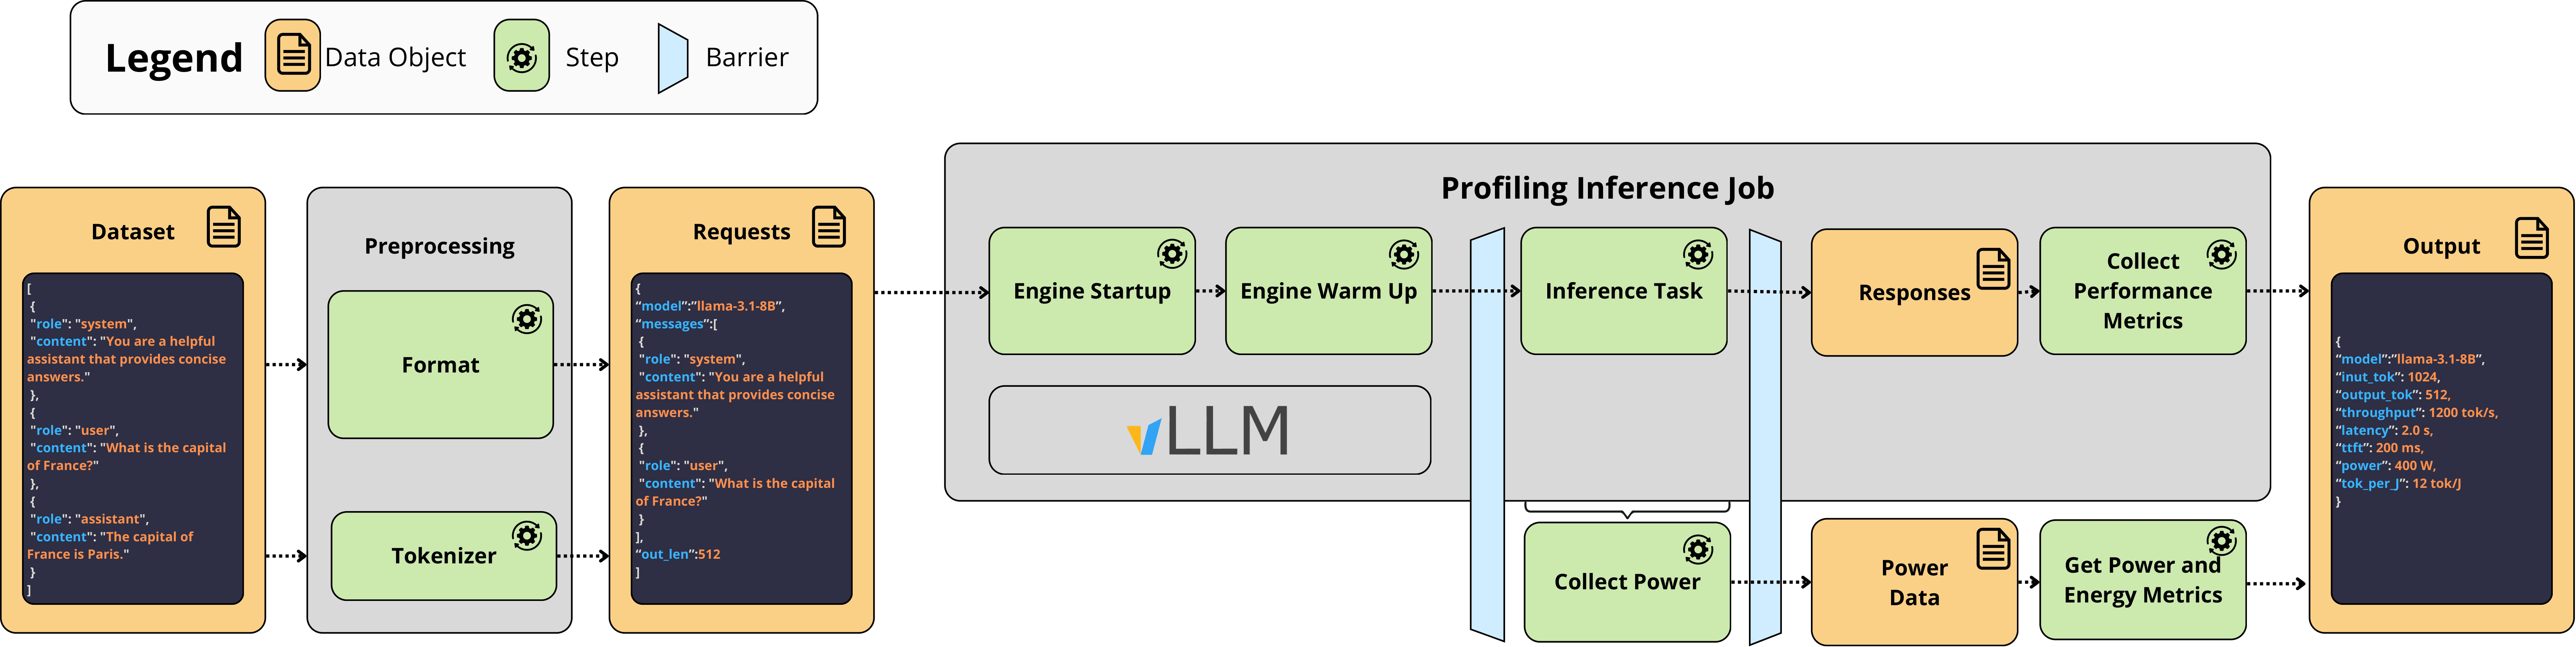
\includegraphics[width=\textwidth]{figs/profile single.png}
    \vspace{5mm}
    \caption{LLM Inference Benchmark Stages.}
    \tagpdfsetup{alttext={LLM Inference Benchmark Stages.}}
    \label{fig:bench}
\end{figure}

To fairly compare those devices, we use a similar software stack on each machine. In particular, we use vLLM \cite{kwon2023efficient}, a high-performance, open-source LLM inference framework compatible with Nvidia, AMD, and Intel GPUs. vLLM allows to achieve superior performance and energy efficiency \cite{fernandez2025energy} compared to the standard Transformers \cite{wolf2019huggingface} implementation by leveraging some key optimizations like the FlashAttention Backend \cite{dao2022flashattention}, PagedAttention \cite{kwon2023efficient}, and continuous batching \cite{agrawal2023sarathi}.
\ref{tab:nodes} reports the specific software stack used on each machine, including the GPU driver, PyTorch version, and vLLM version.

\begin{table}[h!]
\centering
\footnotesize
\caption{GPU nodes used in the experimental evaluation.}
\label{tab:nodes}

\begin{tabularx}{\textwidth}{l l c c c X}
\toprule
\textbf{Vendor} & \textbf{Name} & \textbf{Precision} & \textbf{GPUs/Node} & \textbf{Driver} & \textbf{Software} \\
\midrule

\textbf{NVIDIA} & \textbf{A100}  & BF16, W8A16 & 8  & CUDA 12.6 & \makecell[l]{Torch 2.7.0 \\ vLLM 0.9.0} \\

\textbf{NVIDIA} & \textbf{H100}  & BF16, W8A8  & 4  & CUDA 12.6 & \makecell[l]{Torch 2.7.0 \\ vLLM 0.9.0} \\

\textbf{NVIDIA} & \textbf{GH200} & BF16, W8A8  & 1  & CUDA 12.9 & \makecell[l]{Torch 2.7.0 \\ vLLM 0.9.0} \\

\midrule

\textbf{AMD} & \textbf{MI250}  & BF16        & 4 & ROCm 5.3 & \makecell[l]{Torch 2.7.0+rocm \\ vLLM 0.9.1} \\

\textbf{AMD} & \textbf{MI300X} & BF16, W8A8  & 8 & ROCm 5.3 & \makecell[l]{Torch 2.7.0+rocm \\ vLLM 0.9.1} \\

\midrule

\textbf{Intel} & \textbf{MAX 1550} & FP16 & 6 & oneAPI 2025.2.0 & \makecell[l]{Torch 2.8.0a0 \\ vLLM 0.10.1.xpu} \\

\bottomrule
\end{tabularx}
\end{table}

Each experiment starts by initializing the vLLM engine and loading the inference dataset.
Once the model is loaded and the inference engine is ready, we create an independence process that probes the vendor system monitoring interfaces (py3nvml for NVIDIA, amdsmi for AMD, and xpu-smi for Intel) at consistent intervals to capture power consumption, memory usage, and GPU utilization. For NVIDIA and AMD devices, we sample every 0.5 seconds. For Intel, we have an average sampling rate of 1.9 seconds, due to the longer response time of xpu-smi.
We created the profiler and submitted the inference dataset as a unique batch job to the engine using the vLLM chat method.
Once vLLM has generated the replies for each entry of the dataset, it returns an output object containing information about the end-to-end latency, time to first token, and input and output length of each sequence. This information allows us to collect all the performance metrics described in Section \ref{chap:methods:sec:metrics}.
The profiler data, on the other hand, is used to collect power and energy consumption. To ensure that the profiler process probes the GPU's SMIs only when the GPU is active, we synchronize it with the main process using Python multiprocessing barriers.

For each GPU, this experiment uses different models, precisions, and batch sizes.

Concerning the models, we us four open-source models with a size that ranges from 8B to 32B parameters. Precisely, Llama 3.1 8B, Qwen3 14B, Mistral Small 3.1 24B, and Qwen3 32B. The architectural details of those models are reported in \ref{tab:models}, in the next section.

To evaluate different precisions, we rely on vLLM dynamic weight quantization, which allows us to perform W8A16 quantization (8-bit weights and 16-bit activations) or W8A8 quantization (8-bit weights and 8-bit activations) \cite{vllm-fp8-docs-v0_5_4}, depending on the hardware architecture.
On NVIDIA H100 and AMD MI300x, which offer in-hardware support for FP8 quantization, we use W8A8 quantization. On Nvidia A100, instead, we employ W8A16. Other devices are not included in those experiments, as they do not support either.
For the 16-bit precision, we use bfloat16 (Brain Float 16) precision on Nvidia and AMD, as it is the default precision of the models. For Intel instead, we convert to FP16; single-key optimizations are not yet supported for bfloat16 precision.
Finally, we repeat each experiment for batch sizes of 16 to 128.
\subsection{Multi GPU Experiments}
\label{chap:methods:sec:multi}

We further evaluate LLM inference on GPUs by scaling out to multi-GPU inference.

Multi-GPU parallelism allows for expanding the evaluation in two directions: first, it enables evaluation of significantly larger models compared to single-GPU, thanks to model weight sharding across devices. This also allows a further study of performance scaling with model size. To do so, we include all the models presented in \ref{tab:models}.
Second, as discussed in Section \ref{chap:background:sec:serving}, multi-GPU inference can be implemented using several parallelization strategies, including Tensor Parallelism, Expert Parallelism, and Data Parallelism. As detailed in Section \ref{chap:methods:sec:multi}, these techniques increase the system’s parallel throughput and memory bandwidth approximately linearly with the number of accelerators. Combining these methods introduces a trade-off between the lower communication overhead of Data Parallelism and the greater available memory provided by Tensor Parallelism.

\begin{figure}[h!]
    \centering
    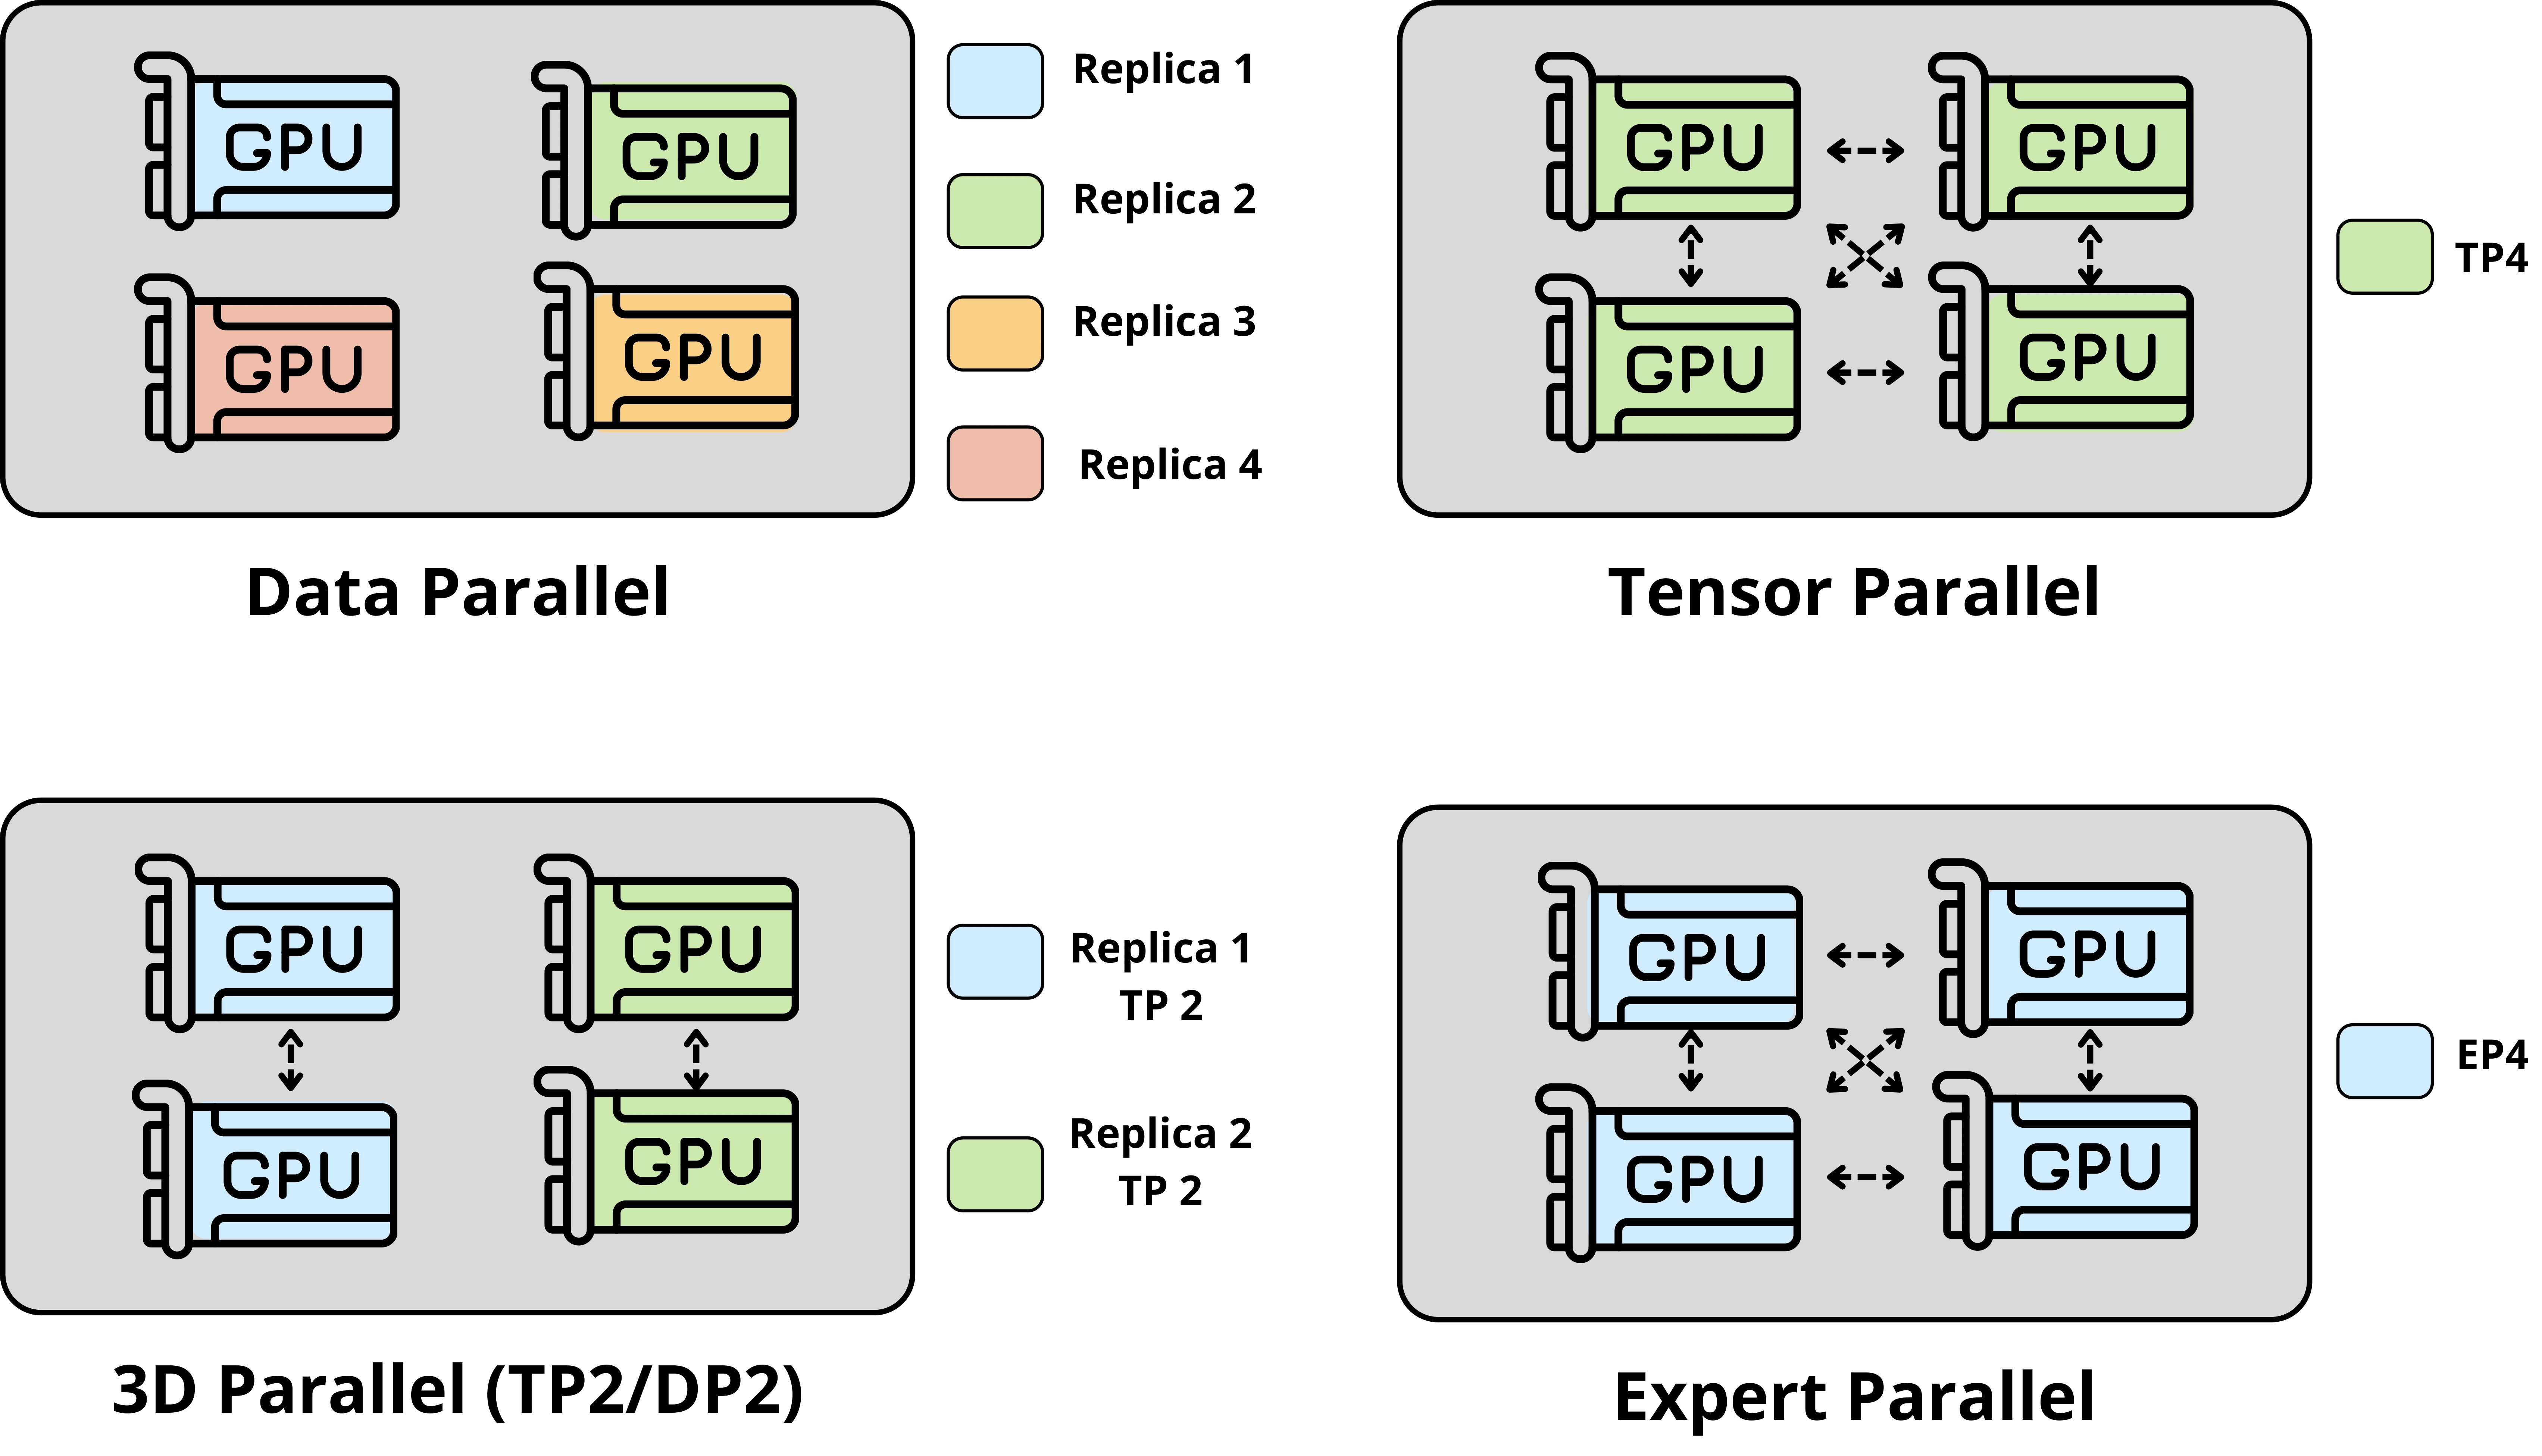
\includegraphics[width=0.85\textwidth]{figs/partition.png}
    \vspace{5mm}
    \caption{Partitioning a node with 3D parallelism.}
    \tagpdfsetup{alttext={Partitioning a node with 3D parallelism.}}
    \label{fig:partition}
\end{figure}

Achieving optimal node-level performance thus requires balancing the number of Data Parallel (DP) replicas and the Tensor Parallel (TP) width per instance, depending on the model size and hardware characteristics. In this study, we explore various TP/DP configurations to empirically determine near-optimal settings. \ref{fig:partition} shows multiple options for partitioning the resources of a 4-GPU node.

\begin{figure}[h!]
    \centering
    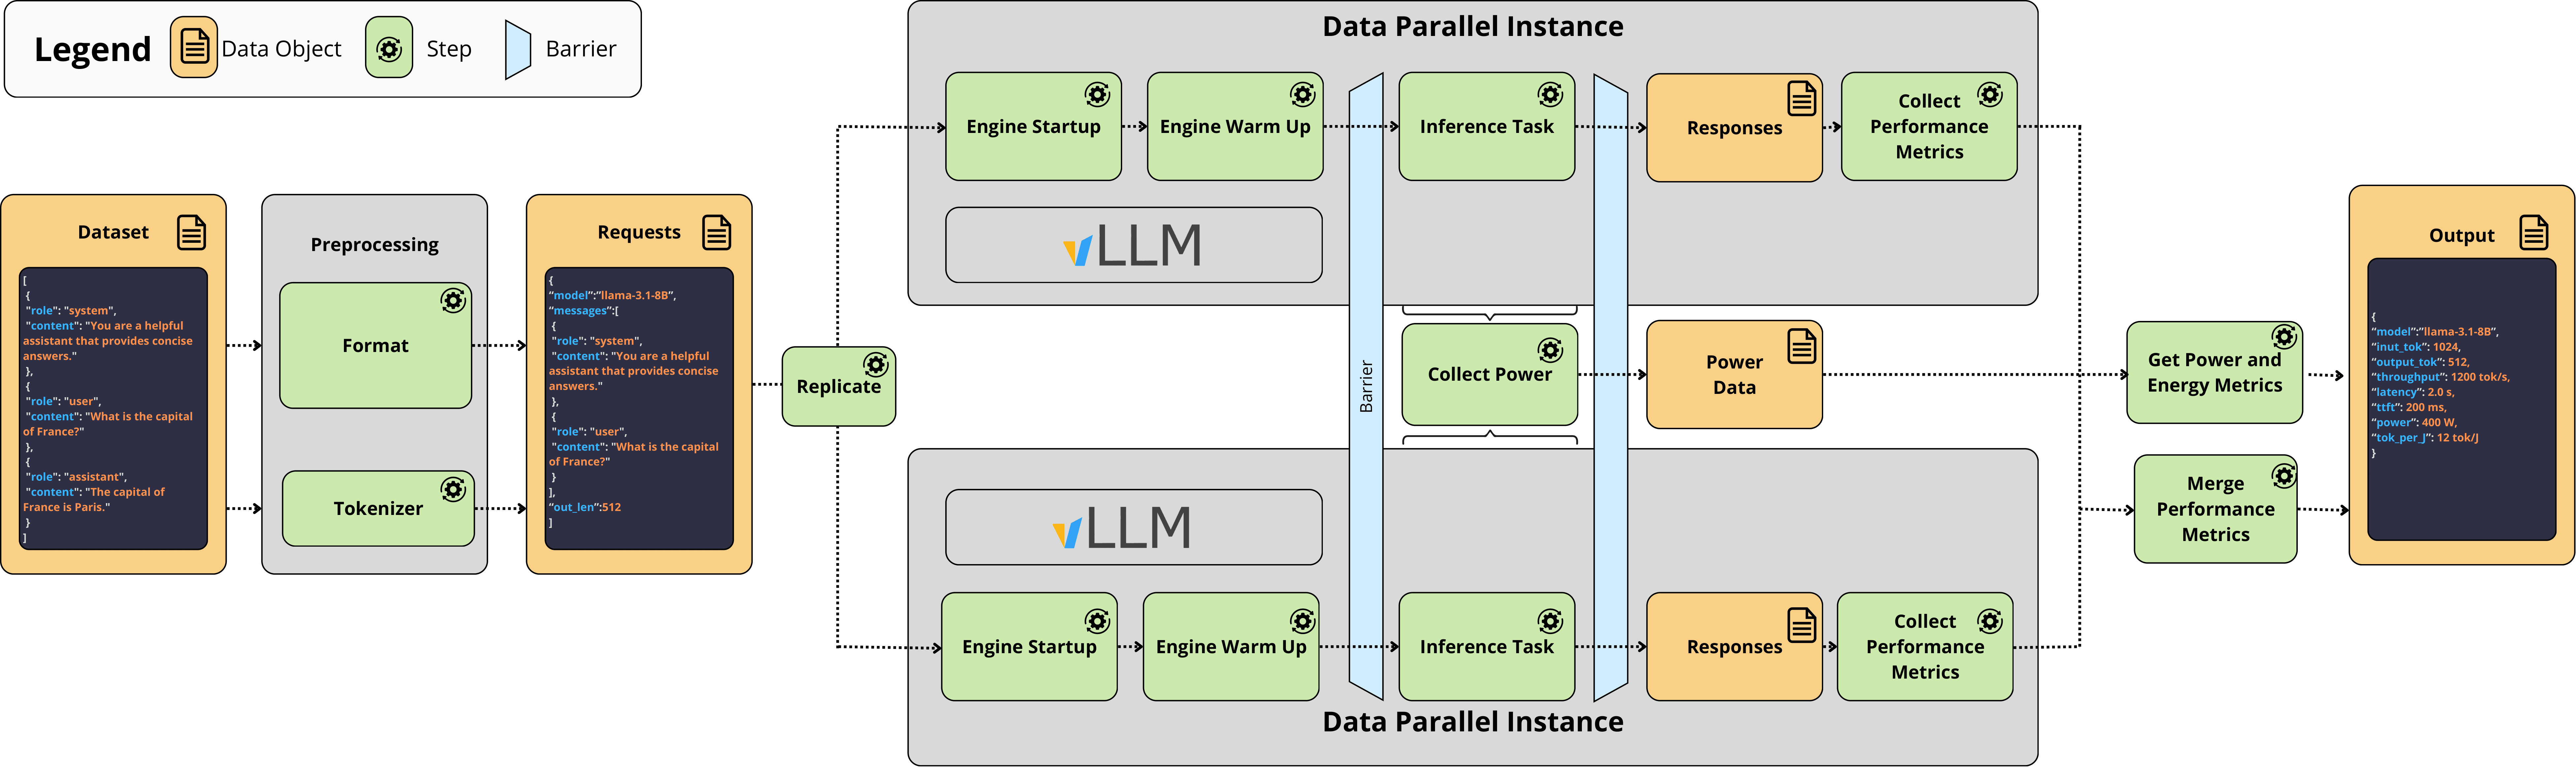
\includegraphics[width=\textwidth]{figs/profile multi.png}
    \vspace{5mm}
    \caption{LLM Inference Benchmark Stages. Multi-GPU setup.}
    \tagpdfsetup{alttext={LLM Inference Benchmark Stages. Multi-GPU setup.}}
    \label{fig:bench}
\end{figure}

An experiment with Data Paralle Size $D$ and Tensor Parallel Size $T$ begins by creating $D$ worker processes and one profiler process. Similar to the single-GPU setup, the profiler process probes the vendor-specific system monitoring interface at consistent intervals to retrieve power consumption data.
Each worker process, instead, initiates a vLLM instance with Tensor Parallel Size $T$. Setting $T\times D = N$, where $N$ is the number of GPUs of the node, allows for an even partition into $D$ homogenous portions, as shown by \ref{fig:partition}.

Once all the $D$ instances are ready, each one starts processing a full instance of the dataset, scaling the single-GPU experiment weakly. When all instances have finished generating replies, their outputs are combined to extract performance metrics, and the profiler process is terminated.

We repeat this experiment with Tensor Parallel Size $T \in \{1, 2, 4\}$ on three multi-GPU nodes: one Sophia bigmem node, featuring 8 DGX A100 80GB GPUs, and two JLSE testbed nodes, featuring 4 NVIDIA H100 SXM5 and 8 AMD Instinct MI300X, respectively. The Data Parallel Size $D$ is set to fully utilize the node. 
The global batch size is set to $128 \times N$, meaning that each of the $D$ instances has a batch size of $128\times T$.
We evaluate both bfloat16 precision and FP8 quantization, using W8A8 on Nvidia H100 and AMD MI300x, and W8A16 on Nvidia A100.

These weak scaling settings allow us to have cleaner performance scaling in two ways. First, it maintains consistency in context lengths across data-parallel instances, since all replicas process identical sequences. Second, it maintains a constant batch size per GPU, ensuring that the number of generated tokens per forward pass remains unchanged across different TP/DP configurations.

\subsection{Comparing Tensor and Expert Parallelism}

We further investigate parallelization strategies for Mixture-of-Experts (MoE) models by comparing Tensor Parallelism (TP) and Expert Parallelism (EP).

Our evaluation includes four large MoE models — Llama4 Scout, Mixtral 8×22B, Qwen 235B A22B, and DeepSeek R1 — all tested in FP8 precision on NVIDIA H100 and AMD MI300x nodes.

Experiments are conducted across varying batch sizes, using a single instance (Data Parallel size = 1) with four GPUs per instance. We first test with a Tensor Parallel size of 4, followed by an Expert Parallel size of 4. The profiling methods used are consistent with those employed in the previous experiment. For DeepSeekR1, we also experimented with 8 GPUs.

\subsection{Dataflow Accelerators Experiments}
\label{chap:methods:sec:dsa}

We investigate LLM inference on hardware accelerators using two dataflow machines: a SambaNova Systems SN40L-16R node \cite{Prabhakar2024}, featuring 16 4th-generation RDUs, and a Cerebras CS3 system \cite{Lie2023} featuring the third-generation Wafer Scale Engine (WSE3). The details of those accelerators are discussed in Section \ref{chap:background:sec:dflow}.

While GPUs are characterized by many streaming multiprocessors that share a common hierarchical memory, dataflow accelerators feature a tiled array of interconnected processing elements, allowing for the mapping of computational graphs into the hardware fabric. This dataflow approach enables reliance solely on fast local scratchpad memories and explicit communication between cores, rather than using a hierarchical cache system as in GPUs, thereby reducing the latency of memory accesses.

Unlike the GPU experiments, which all leveraged vLLM, we utilize a different proprietary inference framework for each dataflow accelerator.

For the Cerebras CS3 system, we use an early-prototype proprietary inference engine that can be queried through an OpenAI-style API.
We task the engine with processing the entire inference dataset by creating one request per conversation.
The Cerebras inference engine supports running models that host weights, activations, and KV caches entirely in on-chip memory to achieve optimal performance. Compared to the streaming-weight approach used for training, this limits the memory capacity to 44GB per CS3 system. For this reason, we limit our analysis to  Llama 3.1 8B.

We repeat the experiment for different batch sizes, ranging from 1 to 8.
To match the engine's effective batch size, we instantiate a corresponding number of clients that send a new request immediately after receiving a response, with the dataset evenly partitioned across clients.
The latencies reported in the responses sent to clients are used to obtain performance metrics.

Regarding power, we collect measurements at the WSE chassis level for all power readings, including the power drawn by the host CPU, WSE, and other supporting components.

For the SambaNova SN40L, we use the SambaStudio inference engine, which can be queried through an OpenAI-compatible interface. Similar to the Cerebras CS3 experiments, we evaluate batch sizes from 1 to 8, creating a number of clients to match the engine's effective batch size.
For this accelerator, we evaluate both Llama 3.1 8B and Llama 3.3 70B.

Regarding power readings, we rely on the PDU-level power consumption for each RDU.